\section{ESTRUTURAS DE DADOS E ESTRATÉGIAS DE IMPLEMENTAÇÃO}
\label{sec:estruturasDadosEstrategiasImplementacao}

À implementação do sistema de simulação são empregadas estruturas de dados puramente vetoriais armazenadas em espaços de memória contíguos no computador. A motivação do uso de estruturas vetoriais advém do fato de que reduzem a complexidade estrutural no código-fonte e viabilizam a posterior paralelização em CUDA facilitando os processos de cópia de dados entre CPU e GPU. Estruturas dinâmicas complexas, que suportam quantidades variáveis de elementos e garantem maior flexibilidade ao programador, são desencorajadas por serem de difícil trato às operações de cópia de dados entre dispositivos e necessitarem de métodos específicos para serialização e desserialização de dados, que acarretam em aumento na carga de processamento e tempo de implementação. 

O processo de vetorização das estruturas de dados, isto é, a redução de estruturas n-dimensionais em unidimensionais, somente é possível graças à manutenção da simplicidade dos agentes e das estruturas de dados empregadas aos ambientes utilizados em simulações, em que é possível realizar o armazenamento e posterior interpretação de seus dados por meio do uso de vetores de tipo homogêneo e com quantidade fixa de elementos. 

À redução do consumo de memória do sistema de simulação, os vértices do grafos que representam as posições do ambiente não armazenam quaisquer informações sobre os agentes que as ocupam. Quando necessário realizar a coleta dos agentes que ocupam uma determinada posição, o vetor de agentes é percorrido em limites definido por índices auxiliares. Como os vetores dos agentes são constantemente processados durante a simulação, os índices auxiliam na redução do espaço de busca dos agentes que estão em determinada posição. Os índices descrevem quais posições dos vetores de agentes devem ser percorridas para encontrar os agentes que estão em uma determinada quadra. Deste modo, os vetores de agentes são constantemente ordenados durante a simulação, utilizando com chave de ordenação o campo de quadra dos agentes. Interior a cada grupo, as buscas são realizadas sequencialmente.

A relação de vizinhança entre os vértices do ambiente é descrita semelhantemente à forma utilizada para a descrição das arestas de um grafo, especificando-se os vértices de origem e destino. A estrutura de grafo utilizada é ilustrada na Figura \ref{fig:grafo}. Não são considerados pesos nas arestas, que são empregadas unicamente para descrever as relações de adjacência entre as vértices. A cada vértice do ambiente são associados quatro identificadores, os identificadores únicos da quadra, do lote, e as coordenadas da latitude e longitude do ponto georreferenciado. As coordenadas da latitude e longitude do ponto são truncadas, sendo eliminadas suas partes fracionárias antes do armazenamento no agente. Os identificadores únicos das quadras e dos lotes são atribuídos de forma sequencial em rotinas de pré-processamento, de forma que sejam únicos para as quadras e para os lotes. Os identificadores dos lotes são únicos para lotes pertencentes à uma mesma quadra, mas se repetem entre lotes pertencentes à diferentes quadras.

\begin{figure}[H]
  \centering
  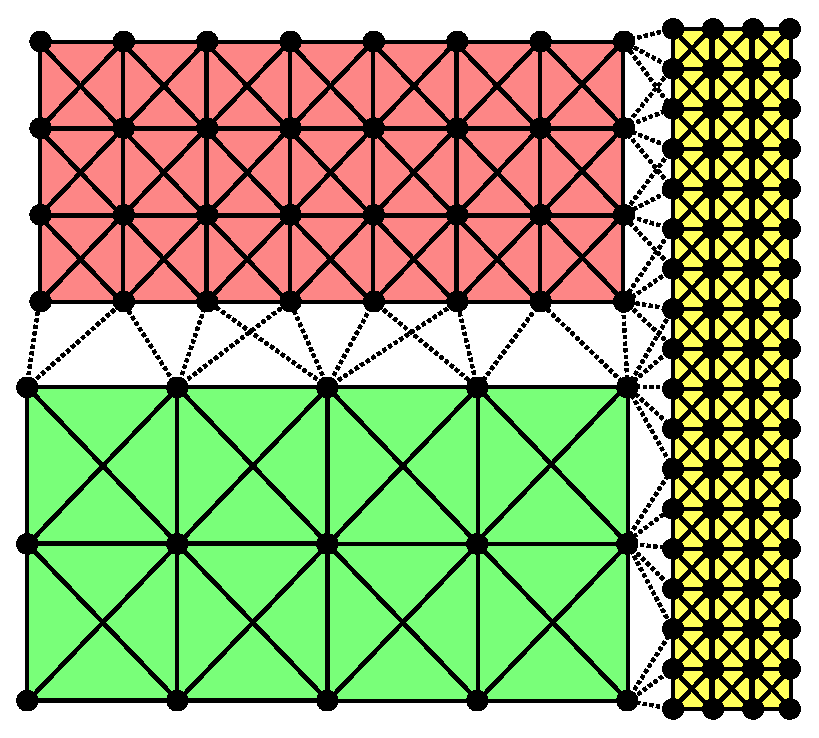
\includegraphics[width=0.38\textwidth]{Figuras/EstruturasDadosEstrategias/grafo.eps}
  \caption{Ilustração da estrutura em grafos empregada para a representação do mapeamento lógico dos lotes e quadras}
  \label{fig:grafo}
\end{figure} 

Quanto à implementação empregando a técnica de \textit{bitstring}, as alterações que precisam ser realizadas em termos de estruturas de dados são mínimas. Necessita-se somente alterar os métodos de manipulação de atributos de forma que operem sobre faixas específicas de \textit{bits} das palavras. As operações \textit{bitstring} empregadas nesta modelagem são aquelas descritas na Seção \ref{sec:modelagemBitstring}.

No Algoritmo \ref{alg:rotina_principal} e Fluxograma \ref{fig:rotina_principal} são ilustrados o algoritmo e fluxograma das principais operações realizadas durante a simulação, bem como sua ordem de execução. 

\newpage

\begin{algorithm}[H]
 \SetAlgoLined
 \input{Codigos/EstruturasDadosEstrategias/Algoritmos/main.txt}
 \caption{\textsc{Principais operações executadas durante a simulação}} 
 \label{alg:rotina_principal}
\end{algorithm}

\begin{figure}[H]
  \centering
  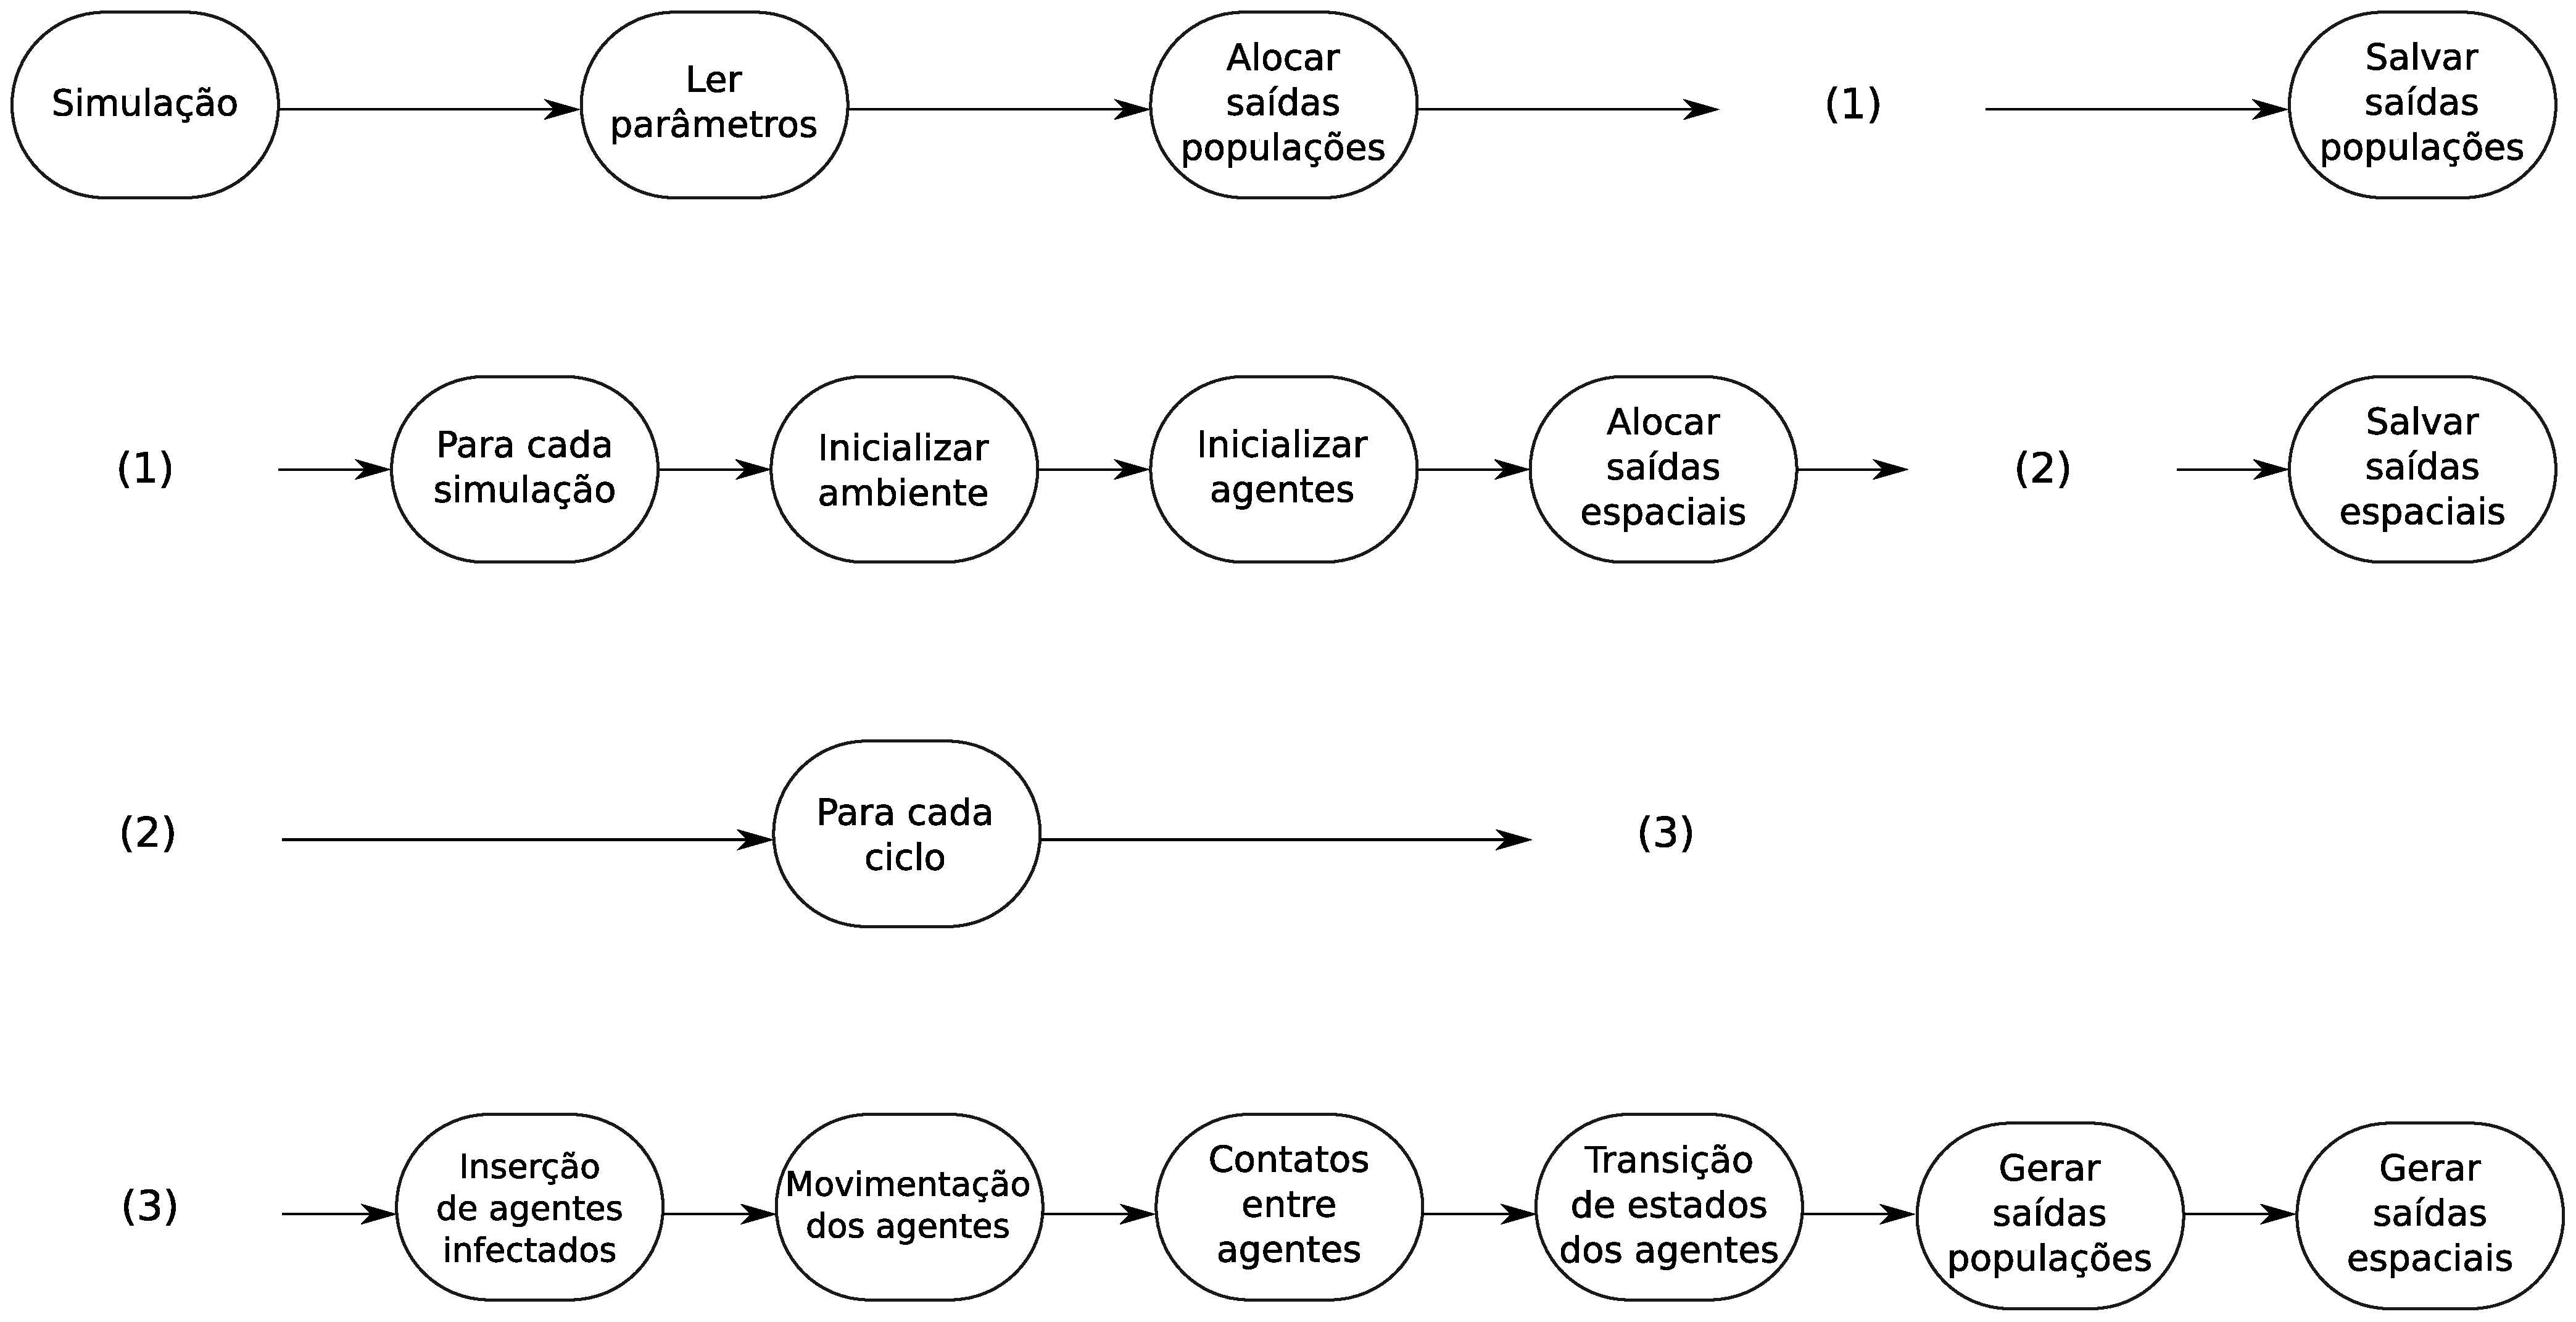
\includegraphics[width=0.9\textwidth]{Figuras/EstruturasDadosEstrategias/main.eps}
  \caption{Fluxograma das principais operações executadas durante a simulação}
  \label{fig:rotina_principal}
\end{figure} 

Nas próximas sub-seções são apresentados os códigos, algoritmos e fluxogramas para todos os operadores aplicados sobre a população de agentes, que são a movimentação, contato e transição. 

\newpage

\subsection{Operações aos Agentes}

\subsubsection{Movimentação}

Nesta operação os agentes são movimentados no ambiente computacional para posições vizinhas escolhidas aleatoriamente, exceto aquelas agentes em quarentena, que são movidos localmente em seu lote atual. Adicionalmente, uma fração dos agentes infectantes são movimentados (migração) para posições aleatórias do ambiente, que não necessariamente pertençam à sua vizinhança, com o objetivo de mimetizar redes de mundo pequeno. A rotina de movimentação dos agentes é ilustrada no Código \ref{cod:movimentacao}, Algoritmo \ref{alg:movimentacao} e Figura \ref{fig:movimentacao}.  

\lstinputlisting[caption=Função Movimentação, label=cod:movimentacao, captionpos=b, language=C++]{Codigos/EstruturasDadosEstrategias/Fontes/Movimentacao.cu}

\begin{algorithm}[H]
  \SetAlgoLined   
  \input{Codigos/EstruturasDadosEstrategias/Algoritmos/Movimentacao.txt}
  \caption{\textsc{Movimentação dos agentes}}
  \label{alg:movimentacao}
\end{algorithm}

\begin{figure}[H]
  \centering
  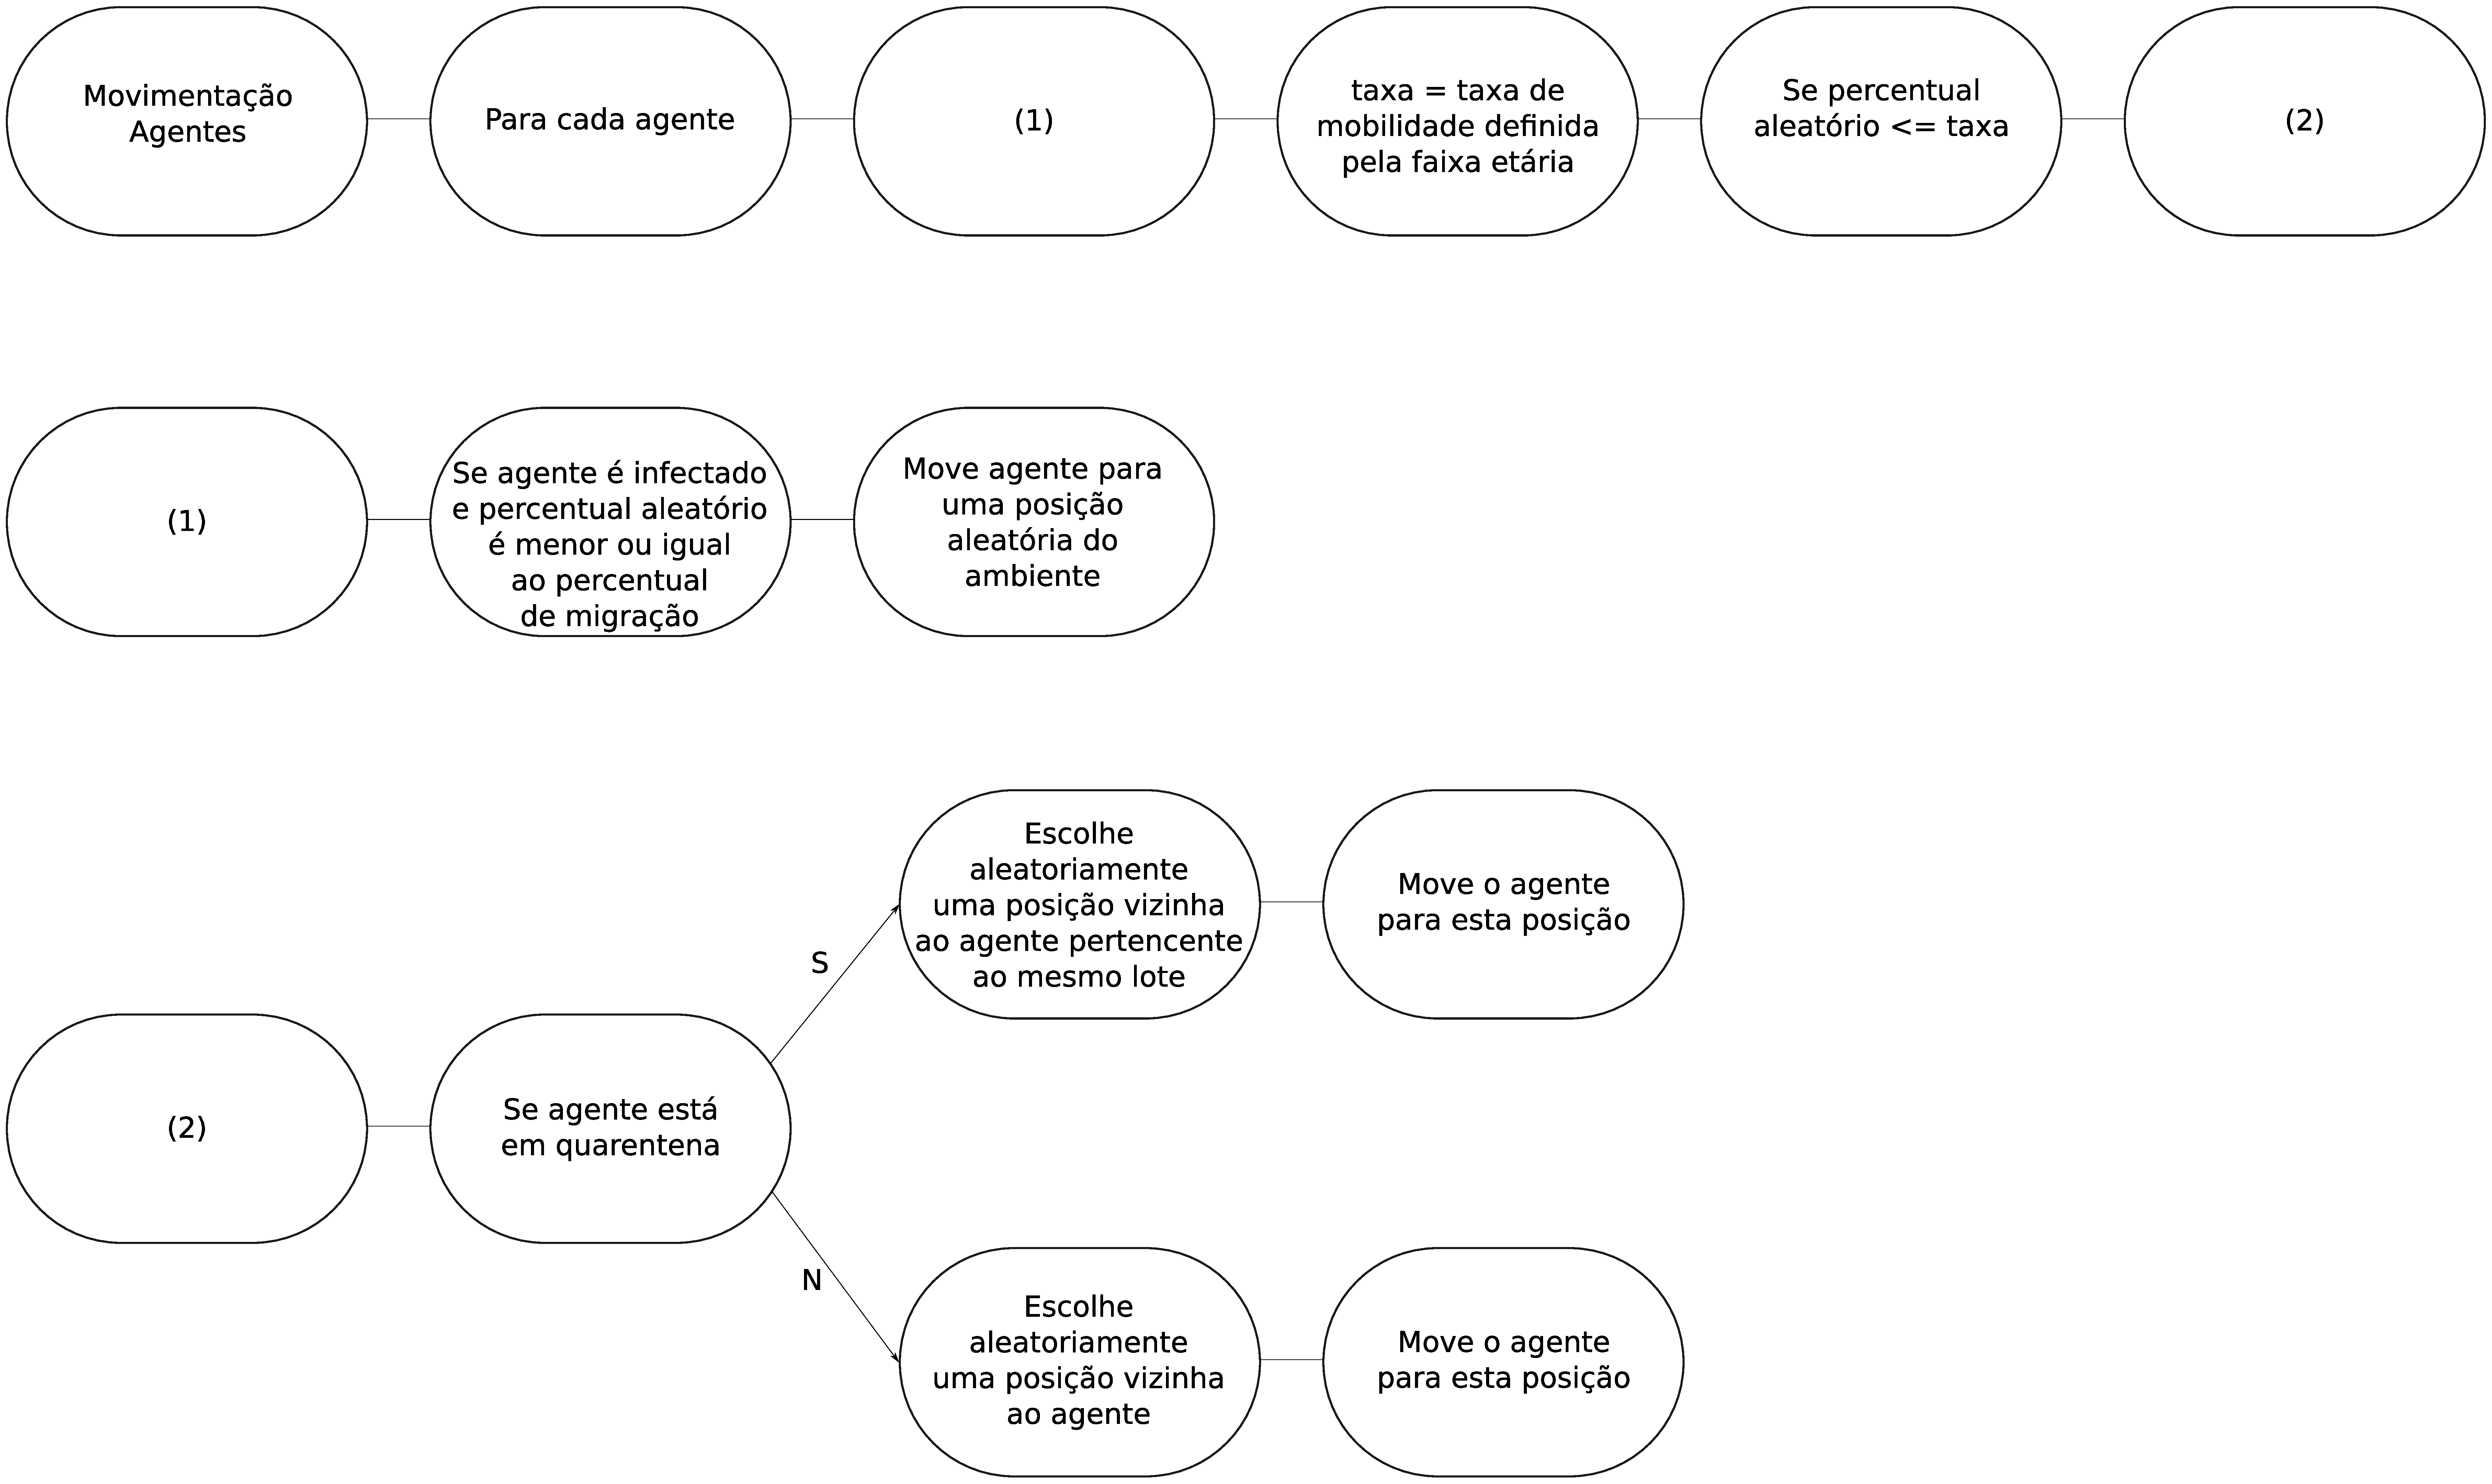
\includegraphics[width=0.95\textwidth]{Figuras/EstruturasDadosEstrategias/Operadores/Movimentacao.eps}
  \caption{Função Movimentação}
  \label{fig:movimentacao}
\end{figure} 

\newpage

\subsubsection{Contato}

Nesta operação são realizados os contatos entre agentes, em que ocorrem a transmissão da doença. A rotina de contato é ilustrada no Código \ref{cod:contato}, Algoritmo \ref{alg:contato} e Figura \ref{fig:contato}. 

\lstinputlisting[caption=Função Contato, label=cod:contato, captionpos=b, language=C++]{Codigos/EstruturasDadosEstrategias/Fontes/Contato.cu}

\begin{algorithm}[H]
 \SetAlgoLined  
 \input{Codigos/EstruturasDadosEstrategias/Algoritmos/Contato.txt}
 \caption{\textsc{Função Contato}} 
 \label{alg:contato}
\end{algorithm}

\begin{figure}[H]
  \centering
  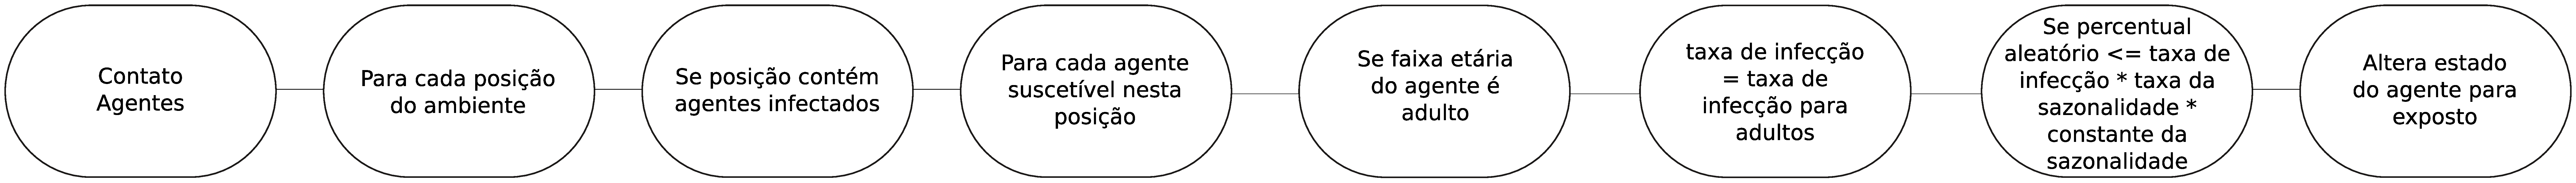
\includegraphics[width=1\textwidth]{Figuras/EstruturasDadosEstrategias/Operadores/Contato.eps}
  \caption{Função Contato}
  \label{fig:contato}
\end{figure} 

\newpage

\subsubsection{Transição}

\subsubsubsection{Transição de Estados}

Nesta operação são realizadas as transições de estados, vacinação e quarentena dos agentes. Na transição de estados os contadores dos agentes são comparados com os parâmetros que definem seus tempos máximos de permanência nos distintos compartimentos considerados à doença. Quando verificado que o período de permanência do agente no atual compartimento encerrou-se, ele é passado para o próximo compartimento. A rotina de transição de estados dos agentes é ilustrada no Código \ref{cod:transicao}, Algoritmo \ref{alg:transicao} e Figura \ref{fig:transicao}. 

\lstinputlisting[caption=Função Transição, label=cod:transicao, captionpos=b, language=C++]{Codigos/EstruturasDadosEstrategias/Fontes/Transicao.cu}

\begin{algorithm}[H]
 \SetAlgoLined  
 \input{Codigos/EstruturasDadosEstrategias/Algoritmos/Transicao.txt}
 \caption{\textsc{Função Transição}} 
 \label{alg:transicao}
\end{algorithm}

\begin{figure}[H]
  \centering
  
\includegraphics[width=1\textwidth]{Figuras/EstruturasDadosEstrategias/Operadores/Transicao.eps}
  \caption{Função Transição}
  \label{fig:transicao}
\end{figure} 

\subsubsubsection{Vacinação}

Nesta operação são realizadas as vacinações dos agentes. Somente os agentes humanos localizados em quadras com vacinação são vacinados. Além disso, as campanhas de vacinação iniciam-se e permanecem ativas em ciclos de tempos determinados. A fração de agentes vacinados decresce a cada dia da campanha. Os agentes que recebem a vacina podem ser passados ao estado imunizado de acordo com a taxa de eficácia de vacina, que é definida nos parâmetros de simulação. A rotina de vacinação dos agentes é ilustrada no Código \ref{cod:vacinacao}, Algoritmo \ref{alg:vacinacao} e Figura \ref{fig:vacinacao}. 

\lstinputlisting[caption=Função Vacinação, label=cod:vacinacao, captionpos=b, language=C++]{Codigos/EstruturasDadosEstrategias/Fontes/Vacinacao.cu}

\begin{algorithm}[H]
 \SetAlgoLined  
 \input{Codigos/EstruturasDadosEstrategias/Algoritmos/Vacinacao.txt}
 \caption{\textsc{Função Vacinação}} 
 \label{alg:vacinacao}
\end{algorithm}

\begin{figure}[H]
  \centering
  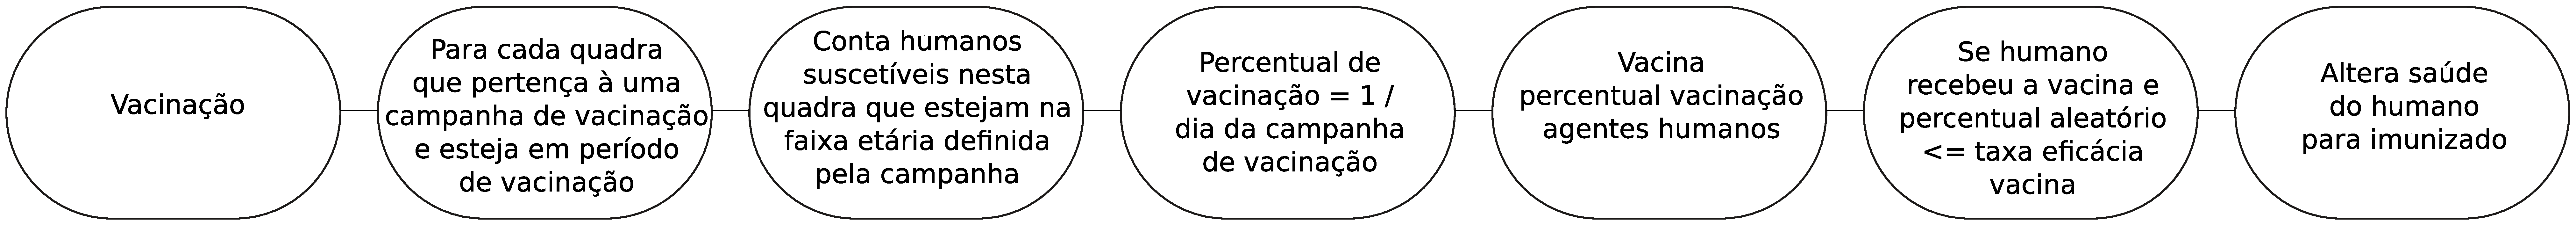
\includegraphics[width=1\textwidth]{Figuras/EstruturasDadosEstrategias/Operadores/Vacinacao.eps}
  \caption{Função Vacinação}
  \label{fig:vacinacao}
\end{figure} 

\subsubsubsection{Quarentena}

Nesta operação são realizadas a passagem dos agentes infectantes ao estado de quarentena, de acordo com probabilidade de transição definida pelo vetor quarentena no ciclo atual de simulação. A rotina de transição à quarentena dos agentes é ilustrada no Código \ref{cod:quarentena}, Algoritmo \ref{alg:quarentena} e Figura \ref{fig:quarentena}. 

\lstinputlisting[caption=Função Quarentena, label=cod:quarentena, captionpos=b, language=C++]{Codigos/EstruturasDadosEstrategias/Fontes/Quarentena.cu}

\begin{algorithm}[H]
 \SetAlgoLined  
 \input{Codigos/EstruturasDadosEstrategias/Algoritmos/Quarentena.txt}
 \caption{\textsc{Função Quarentena}} 
 \label{alg:quarentena}
\end{algorithm}

\begin{figure}[H]
  \centering
  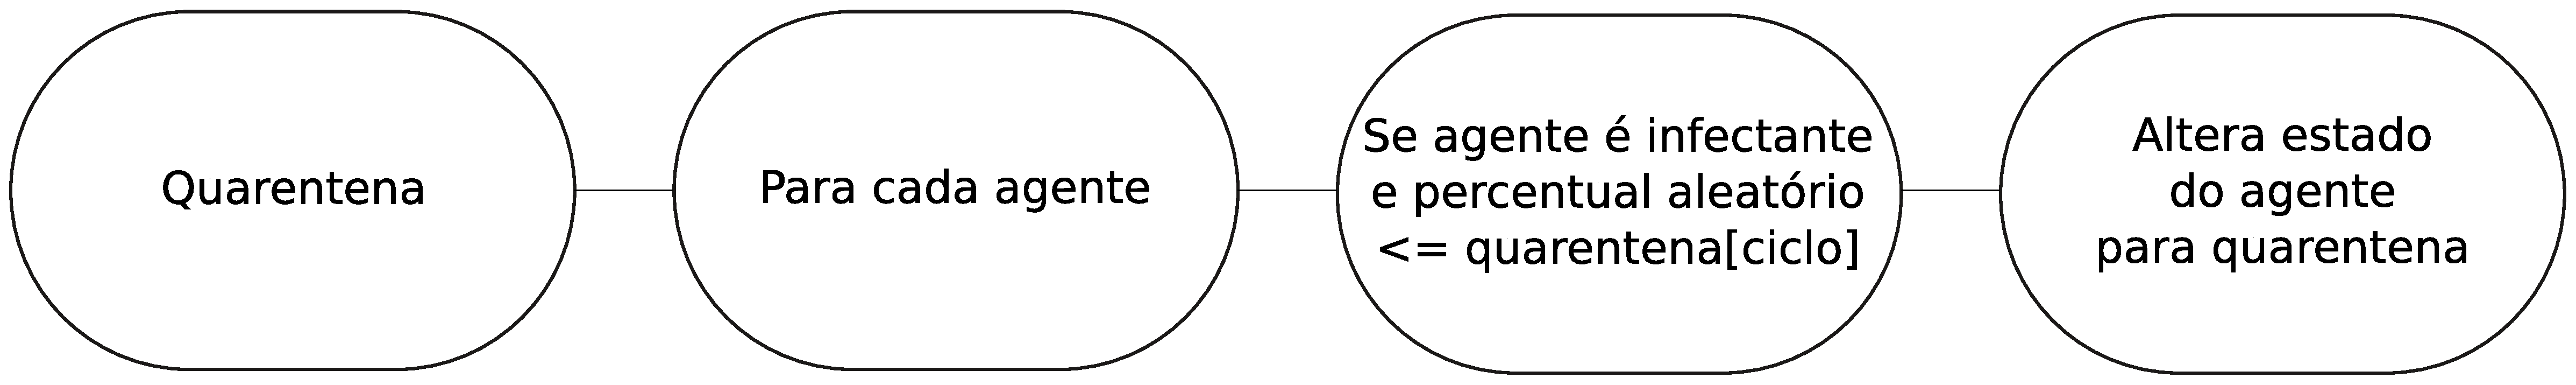
\includegraphics[width=1\textwidth]{Figuras/EstruturasDadosEstrategias/Operadores/Quarentena.eps}
  \caption{Função Quarentena}
  \label{fig:quarentena}
\end{figure} 

A Seção \ref{sec:SIMULA} apresenta o \textit{software} utilizado como apoio às operações de manipulação de dados georreferenciados, que são empregados à geração de arquivos de entrada e visualizações às simulações.

\newpage